% Header mit Deklarationen
\documentclass[
	pdftex,%              PDFTex verwenden
	a4paper,%             A4 Papier
	oneside,%             Einseitig
	bibtotoc,%    		Literaturverzeichnis einf�gen bibtotocnumbered: nummeriert
	liststotoc,%		Verzeichnisse einbinden in toc
	idxtotoc,%            Index ins Verzeichnis einf�gen
	halfparskip,%        Europ�ischer Satz mit abstand zwischen Abs�tzen
	chapterprefix,%       Kapitel anschreiben als Kapitel
	headsepline,%         Linie nach Kopfzeile
	%footsepline,%         Linie vor Fusszeile
	%pointlessnumbers,%     Nummern ohne abschlie�enden Punkt
	12pt%                 Gr�ssere Schrift, besser lesbar am bildschrim
]{scrbook}

%
% Paket fuer Uebersetzungen ins Deutsche
%
\usepackage[ngerman]{babel}

%
% Pakete um Latin1 Zeichnensaetze verwenden zu koennen und die dazu
% passenden Schriften.
%
\usepackage[latin1]{inputenc}
\usepackage[T1]{fontenc}

%
% Paket fuer Quotes
%
\usepackage[babel,french=guillemets,german=swiss]{csquotes}

%
% Paket zum Erweitern der Tabelleneigenschaften
%
\usepackage{array}

%
% Paket fuer schoenere Tabellen
%
\usepackage{booktabs}

%
% Paket um Grafiken einbetten zu koennen
%
\usepackage{graphicx}

%
% Spezielle Schrift im Koma-Script setzen.
%
\setkomafont{sectioning}{\normalfont\bfseries}
\setkomafont{captionlabel}{\normalfont\bfseries} 
\setkomafont{pagehead}{\normalfont\bfseries} % Kopfzeilenschrift
\setkomafont{descriptionlabel}{\normalfont\bfseries}

%
% Zeilenumbruch bei Bildbeschreibungen.
%
\setcapindent{1em}

%
% Kopf und Fusszeilen
%
\usepackage{scrpage2}
\pagestyle{scrheadings}
% Inhalt bis Section rechts und Chapter links
\automark[section]{chapter}
% Mitte: leer
\chead{}

%
% mathematische symbole aus dem AMS Paket.
%
\usepackage{amsmath}
\usepackage{amssymb}

%
% Type 1 Fonts f\"ur bessere darstellung in PDF verwenden.
%
%\usepackage{mathptmx}           % Times + passende Mathefonts
%\usepackage[scaled=.92]{helvet} % skalierte Helvetica als \sfdefault
\usepackage{courier}            % Courier als \ttdefault

%
% Paket um Textteile drehen zu k�nnen
%
\usepackage{rotating}

%
% Paket fuer Farben im PDF
%
\usepackage{color}

%
% Paket fuer Links innerhalb des PDF Dokuments
%
\definecolor{LinkColor}{rgb}{0,0,0.5}
\usepackage[%
	pdftitle={Titel},% Titel der Diplomarbeit
	pdfauthor={Autor},% Autor(en)
	pdfcreator={LaTeX, LaTeX with hyperref and KOMA-Script},% Genutzte Programme
	pdfsubject={Betreff}, % Betreff
	pdfkeywords={Keywords}]{hyperref} % Keywords halt :-)
	
\hypersetup{colorlinks=true,% Definition der Links im PDF File
	linkcolor=LinkColor,%
	citecolor=LinkColor,%
	filecolor=LinkColor,%
	menucolor=LinkColor,%
	pagecolor=LinkColor,%
	urlcolor=LinkColor}

%
% Paket um LIstings sauber zu formatieren.
%
\usepackage[savemem]{listings}
\lstloadlanguages{TeX}

%
% Listing Definationen f�r PHP Code
%
\definecolor{lbcolor}{rgb}{0.85,0.85,0.85}
\lstset{language=[LaTeX]TeX,
	numbers=left,
	stepnumber=1,
	numbersep=5pt,
	numberstyle=\tiny,
	breaklines=true,
	captionpos=b,				% caption-position bottom
	breakautoindent=true,
	postbreak=\space,
	tabsize=2,
	basicstyle=\ttfamily\footnotesize,
	showspaces=false,
	showstringspaces=false,
	extendedchars=true,
	backgroundcolor=\color{lbcolor}}
%
% ---------------------------------------------------------------------------
%


%
% Neue Umgebungen
%
\newenvironment{ListChanges}%
	{\begin{list}{$\diamondsuit$}{}}%
	{\end{list}}

%
% aller Bilder werden im Unterverzeichnis figures gesucht:
%
\graphicspath{{bilder/}}

%
% Literaturverzeichnis-Stil
%
\bibliographystyle{plain}

%
% Anfuehrungsstriche mithilfe von \textss{-anzufuehrendes-}
%
\newcommand{\textss}[1]{"`#1"'}

%
% Strukturiertiefe bis subsubsection{} moeglich
%
\setcounter{secnumdepth}{3}

%
% Dargestellte Strukturiertiefe im Inhaltsverzeichnis
%
\setcounter{tocdepth}{3}

%
% Zeilenabstand wird um den Faktor 1.5 veraendert
%
%\renewcommand{\baselinestretch}{1.5}

%
% Abkuerzungsverzeichnis
%
\usepackage{nomencl}
% Befehl umbenennen in abk
\let\abk\nomenclature
% Deutsche Ueberschrift
\renewcommand{\nomname}{Abk\"urzungsverzeichnis}
% Punkte zw. Abkuerzung und Erklaerung
\setlength{\nomlabelwidth}{.20\hsize}
\renewcommand{\nomlabel}[1]{#1 \dotfill}
% Zeilenabstaende verkleinern
\setlength{\nomitemsep}{-\parsep}
\makenomenclature

\usepackage{eso-pic}
\newcommand\BackgroundPic{%
\put(0,0){%
\parbox[b][\paperheight]{\paperwidth}{%
\vfill
\centering

\includegraphics[width=0.8\paperwidth,height=0.8\paperheight,%
keepaspectratio]{bilder/titelbild.png}%
\vfill
}}}

%
% Kapitelueberschriften werden in eine Zeile geschrieben.
%
% normal: 
% Kapitel 1.
% Einleitung
%
% wenn hier auskommentiert:
% Kapitel 1: Einleitung
%
%\usepackage{titlesec}
%\titleformat{\chapter}[hang] 
%{\normalfont\huge\bfseries}{\chaptertitlename\ \thechapter:}{1em}{} 



\begin{document}
% Hintergrundbild fuer Titelseite einfuegen
% nur bei Titelseite von HTL-Shkoder einkommentieren
% nicht bei Titleseitesimpel
\AddToShipoutPicture*{\BackgroundPic}


% Roemische Nummerierung fuer Sonderseiten, wie Kurzfassung, Abstract, Verzeichnisse und Anhang
\pagenumbering{Roman}

% Titelblatt HTL-Shkoder
% Die Titelseite

\newcommand{\trtitle}{\v{S}koda IT-Support}
\newcommand{\trort}{Shkoder}
\newcommand{\trbetreuer}{DI (FH) Philip MICHEL (Hauptbetreuer)}
\newcommand{\trfachgebiet}{SEW, INSY, NWTK }
\newcommand{\trdate}{\today}
\newcommand{\trnumber}{1504}
\newcommand{\trclass}{5B}
\newcommand{\trschuelereins}{Franc Bushati}
\newcommand{\trschuelerzwei}{Igli Kadija}
\newcommand{\trschuelerdrei}{Alfons Lazri}
\newcommand{\trschuelervier}{Mergim Smajlaj}
\newcommand{\trschuelerfuenf}{Riad Kavaja}
\newcommand{\trsauftraggeber}{\v{S}koda}
\newcommand{\trbetreuereins}{DI(FH) Philip Michel}
\newcommand{\trbetreuerzwei}{Alexander KEMINGER MSc}
\newcommand{\trbetreuerdrei}{Christoph SCHRATT MSc}
\newcommand{\trbetreuervier}{Mag. Anita AIGNER}

\thispagestyle{empty}

\vspace{0.1cm}
\begin{flushleft}
\textbf{\LARGE Diplomarbeit Nr. \trnumber} \\
\LARGE Klasse \trclass{}, Schuljahr 2015/16

\vspace{9cm}
\textbf{\LARGE \trtitle}

\vspace{0.5cm}
\begin{table}[htbp]
\large
\begin{tabular}{cl}
   Ausgef\"uhrt von: & \trschuelereins \\ 
   & \trschuelerzwei \\ 
   & \trschuelerdrei \\ 
    & \trschuelervier \\ 
     & \trschuelerfuenf \\ 
 \end{tabular}
\end{table}
\end{flushleft}

\vspace{0.2cm}
\textbf{Auftraggeber:} \trsauftraggeber

\vspace{0.4cm}
\textbf{Hauptbetreuer:} \trbetreuereins \\
\textbf{Hauptbetreuer Stv.:} \trbetreuerzwei \\
\textbf{Nebenbetreuer:} \trbetreuerdrei \\
%\textbf{Sprachbetreuerin:} \trbetreuervier \\
\newline
\large \trort{}, \today 

\vfill

% einfaches Titelblatt
%% Die Titelseite
% Im folgenden kommen ein paar Variablen, die auszuf�llen sind
% Bisher steht dort nur Musterinhalt
% Au�erdem m�ssen zei Dateien erstellt werden, Bild/Logo/Emblem des Fachgebietes
% sowie der Universit�t

\newcommand{\trtitle}{Titel der Diplomarbeit}
\newcommand{\trort}{Shkoder}
\newcommand{\trbetreuer}{Titel Betreuer}
\newcommand{\trdate}{\today}
\newcommand{\trnumber}{15.xx}
\newcommand{\trclass}{5X}
\newcommand{\trschuelereins}{Sch\"uler1}
\newcommand{\trschuelerzwei}{Sch\"uler2}
\newcommand{\trschuelerdrei}{Sch\"uler3}
\newcommand{\trsauftraggeber}{Herr Max Mustermann oder Firma}
\newcommand{\trbetreuereins}{Lehrer1}
\newcommand{\trbetreuerzwei}{Lehrer2}
\newcommand{\trbetreuerdrei}{Lehrer3}

\thispagestyle{empty}

\begin{center}
  \Large H\"ohere technische Schule f\"ur Informationstechnologie
\end{center}

\begin{center}
  
\includegraphics[scale=0.2]{htllogo} \\
  \textbf{\LARGE \trtitle}
\end{center}
\vspace{1cm}

\begin{flushleft}
\textbf{\LARGE Diplomarbeit Nr. \trnumber} \\
\LARGE Klasse \trclass{}, Schuljahr 2015/16

\begin{table}[htbp]
\Large
\begin{tabular}{cc}
   Ausgef\"uhrt von: & \trschuelereins \\ 
   & \trschuelerzwei \\ 
   & \trschuelerdrei \\ 
 \end{tabular}
\end{table}
\end{flushleft}


\large Projektbetreuer1: \trbetreuereins \\
\large Projektbetreuer2: \trbetreuerzwei \\
\large Projektbetreuer3: \trbetreuerdrei \\
\newline
\large \trort{}, \today

\vfill

% Eidesstattliche Erklaerung
% Die eidesstattliche Erklaerung mit Unterschrift
\chapter*{Eidesstattliche Erkl\"arung}

Wir versichern, dass wir die vorstehende Arbeit selbstst\"andig und ohne fremde Hilfe angefertigt haben. Wir haben uns keiner anderen als der im beigef\"ugten Quellenverzeichnis angegebenen Hilfsmittel bedient. Alle Stellen, die w\"ortlich oder sinngem\"a\ss aus Ver\"offentlichungen entnommen wurden, sind als solche kenntlich gemacht.


\vspace{2.5cm}

\hspace{2cm} Ort, Datum \hfill Unterschrift \hspace{2cm}

\vspace{2cm}

\hspace{2cm} Ort, Datum \hfill Unterschrift \hspace{2cm}

\vspace{2cm}

\hspace{2cm} Ort, Datum \hfill Unterschrift \hspace{2cm}

\vspace{2cm}

\begin{center}
S\"amtliche in dieser Diplomarbeit verwendeten personenbezogenen Bezeichnungen sind geschlechtsneutral zu verstehen.
\end{center}

% Kurzfassung
%
% neue Seite
%
\newpage

%
% Ueberschrift Kurzfassung
%
\section*{Kurzfassung}
Was werden wir tun, um den IT-Support f\"ur die Kostandin Group zu realisieren?

Zuerst bauen wir ein Netzwerk auf, weil es in dieser Firma noch kein funktionierendes Netzwerk gibt.
In der Firma verwenden wir zur Zeit vier Computer, welche nicht in einem gemeinsamen Netzwerk verbunden sind. Diese verwenden wir, um das Netzwerk aufzubauen. Dieses Netzwerk wird die innerbetriebliche Kommunikation erleichtern und Datensicherheit garantieren. Wir konfigurieren einen Switch, falls die Firma in Zukunft mehr PC s an das Netz anschlie\ss{}en will.

Auch ein Lagerprogramm m\"ochten wir installieren. Dazu wird das vorhandene Lagerprogramm auf Tauglichkeit evaluiert, gegebenenfalls erweitert, ansonsten finden wir eine alternative und installieren wir es.
Ein weiteres Programm, das wir installieren, ist ein Bilanzprogramm. Damit soll es f\"ur das Unternehmen m\"oglich sein, seine Ausgaben und Einnahmen, den Umsatz und den Gewinn\"ubersichtlich zu dokumentieren.
Wir installieren auch ein Rechnungsverwaltungsprogramm. Das Programm wird die Quittungen f\"ur die Kunden vorbereitet und dann gedruckt.
Zus\"atzlich erstellen wir eine Webseite, auf der die Firma ihre Produkte und Dienstleistungen bewirbt. F\"ur die Realisierung verwenden wir ein CMS und die Technologien HTML, CSS und PHP.

\color{black} 


% Abstract
%
% neue Seite
%
\newpage

%
% Ueberschrift Abstract
%
\section*{Abstract}
In Shkoder there are a lot of companies that are not very familiar with new
technologies. They do all the work manually. Nowadays, however, this work is mostly
done by computers and new technologies. We offer these companies IT-support to
make their work easier and safer. Riad, one of our colleagues, informed us that
Skoda needs IT support. That's why we came up with the idea to do our thesis based
on a partnership with this company. Through an analysis that we carried out, we
realized that the company needs a network, an inventory program, a balancing
program and a website. In a meeting with the owner of Skoda we discussed about
the opportunity to cooperate with him. As we presented our idea to him, he realized
the possibility of improving procedures in his company and that he should take our
help in consideration.
 


% Danksagung
%
% neue Seite
%
\newpage

%
% Ueberschrift Abstract
%
\section*{Danksagung}
Es gibt viele, die uns bei unserer Diplomarbeit unterst\"utzt haben und ohne deren Hilfe diese Arbeit nicht in dieser Form zustande gekommen w\"are.
An erster Stelle m\"ochten wir uns bei Herrn Philip Michel f\"ur seine intensive Betreuung, seine vielf\"altigen und hilfreichen Ideen und seinen Inspiration bedanken.
Bei Herrn Chritoph Schratt und Herrn Alexander Keminger  m\"ochten wir uns f\"ur ihre Unterst\"utzung und Enthusiasmus bedanken,so wie f\"ur viele interessante und n\"utzliche Beratungen.

Danken m\"ochten wir auch Frau Anita Aigner daf\"ur, dass sie unz\"ahlige Male unsere Diplomarbeit gelesen 
und Gramatikfehler verbessert hat. Weiteres wollen wir auch Frau Margit Br\"uckner f\"ur die English Korrekturen bei dem Antrag und bei der Diplomarbeit.

Wir wollen auch unser Projektauftraggeber bedanken, f\"ur die M\"oglichkeit die er uns gegeben hat.

Am Ende m\"ochten wir noch unserer Schule und nat\"urlich auch Frau Tagini f\"ur die gro{\ss}e Unterst\"utzung danken. 

Nat\"urlich m\"ochten wir uns auch noch bei unseren Eltern und unseren Freunden und Freundinnen, die uns 
immer wieder unterst\"utzt haben, herzlich bedanken.

\vspace{4cm}



% Verzeichnisse
% Kopfzeile links Kapitel, rechts leer
\ihead{\leftmark}
\ohead{}

% Inhaltsverzeichnis, Abbildungsverzeichnis, Tabellenverzeichnis
%
% Inhaltsverzeichnis
%
\tableofcontents

%
% Abbildungsverzeichnis
%
\listoffigures

%
% Tabellenverzeichnis
%
\listoftables



% Merke mir die roemische Seitenzahl in 'roemisch' und setzte Nummerierung 
% auf arabisch fuer die eigentlichen Kapitel
\newpage
\newcounter{roemisch}
\setcounter{roemisch}{\value{page}}
\pagenumbering{arabic}

% Die einzelnen Kapitel
% Kopfzeile: links Kapitel, rechts Sektion
%\ihead{\leftmark}
%\ohead{\rightmark}
%\ihead{\parbox[t][2\baselineskip][t]{\dimexpr\linewidth-2em\relax}{\leftmark}}
%\ohead{\parbox[t][2\baselineskip][t]{20em}{\raggedleft\rightmark}}
\chapter{Allgemeines}
\section{Idee, Thema, Aufgabenstellung}

Riad Kavaja, ein Projektmitglied unserer Diplomarbeitsgruppe, hat uns dar\"uber informiert, dass die Skoda Filiale in Shkodra IT-Support ben\"otigt. Das hat uns auf die Idee gebracht, unsere Diplomarbeit in Partnerschaft mit diesem Unternehmen Kostandin Group zu realisieren.
Durch eine Bedarfsanalyse, die wir durchgef\"uhrt haben, konnten wir schlussfolgern, dass die Firma einen Netzaufbau f\"ur ihre Computer, eine Homepage, ein Lagerprogramm, ein Rechnungsverwaltungsprogramm und ein Bilanzprogramm braucht.
Bei einer Besprechung mit dem Gesch\"aftsf\"uhrer von Skoda konnten wir die M\"oglichkeit einer Zusammenarbeit diskutieren. Als wir ihm unsere Idee vorgestellt haben, hat er eingesehen dass in seinem Betrieb ein Verbesserungspotential besteht  und dass er unsere Hilfe in Anspruch nehmen k\"onnte.

\subsection{Beschreibung der Idee}

Was werden wir tun, um den IT-Support f\"ur die Kostandin Group zu realisieren?

Zuerst werden wir ein Netzwerk aufbauen, weil es in dieser Firma noch kein funktionierendes Netzwerk gibt.
In der Firma werden zur Zeit vier Computer verwendet, welche nicht in einem gemeinsamen Netzwerk verbunden sind. Diese werden wir verwenden, um das Netzwerk aufzubauen. Dieses Netzwerk wird die innerbetriebliche Kommunikation erleichtern und Datensicherheit garantieren.Wir werden einen Switch konfigurieren, falls die Firma in Zukunft mehr PC s an das Netz anschliessen will.

Auch ein Lagerprogramm m\"ochten wir installieren. Dazu wird das vorhandene Lagerprogramm auf Tauglichkeit evaluiert, gegebenenfalls erweitert, ansonsten werden wir eine alternative finden und installieren.
Ein weiteres Programm, das wir installieren werden, ist ein Bilanzprogramm. Damit soll es f\"ur das Unternehmen m\"oglich sein, seine Ausgaben und Einnahmen, den Umsatz und den Gewinn \"ubersichtlich zu dokumentieren.
Es wird auch ein Rechnungsverwaltungsprogramm installiert. Das Programm wird die Quittungen f\"ur die Kunden vorbereiten und dann drucken k\"onnen. 

Zus\"atzlich werden wir eine Webseite erstellen, auf der die Firma ihre Produkte und Dienstleistungen bewirbt. F\"ur die Realisierung werden wir ein CMS verwenden und die Technologien HTML, CSS und PHP verwenden.



\chapter{Planung}
\section{Projektziele}
\subsection{MUSS-Ziele}

\subsubsection{Netzwerk aufbauen}
Eines unserer Ziele ist es, ein funktionierendes und erweiterbares Netzwerk aufzubauen. Benutzerprofile, Netzlaufwerke und ein FTP-Zugang werden am Server eingerichtet, um die Kommunikation der Mitarbeiter untereinander zu erleichtern. Somit k\"onnen die Mitarbeiter ihre Dateien zentral abspeichern und miteinander teilen.

\subsubsection{Installation und Inbetriebnahme eines Lagerprogramms und eines Rechnungsmanager, sowie die Einschulung der Mitarbeiter der Firma Skoda}
Damit kein Warenbestand verloren gehen kann (Schwund) und es eine automatische Kontrolle \"uber den aktuellen Lagerbestand gibt (Zufl\"usse und Abfl\"usse), werden wir das aktuelle Lagerverwaltungsprogramm verbessern. Am Ende unseres Projekts wird das Unternehmen nicht wie bisher alle Rechnungen mit Excel erstellen m\"ussen, sondern kann auf ein Programm mit einer Datenbank zur\"uckgreifen. Das erleichtert die Arbeit und Kontrolle der Buchhaltung. Das Rechnungsprogramm soll mit der Datenbank des Lagerprogramms auf den Bestand zugreifen k\"onnen.
Damit die Mitarbeiter mit den neuen Programmen arbeiten k\"onnen, soll ein Benutzerhandbuch erstellt werden, welches in einer Einschulung den Mitarbeitern erkl\"art und vorgestellt wird.

\subsubsection{Hotspot}
Zu Werbezwecken wird f\"ur die Firma ein gratis Hotspot eingerichtet. Beim Verbinden mit dem Hotspot \"offnet sich als Startseite die aktuelle Firmenseite. 


\subsection{Optionale-Ziele (Soll-, Kann-Ziele)}

\subsubsection{Erstellung einer Webseite, Soziale Medien pflegen und verbessern}
Damit diese Firma \"uberall in Shkodra und auch ausserhalb bekannt wird, muss sie eine gute Internet-Werbung haben. Deshalb werden wir f\"ur das Unternehmen eine Webseite in Wordpress erstellen und auch die sozialen Netze bewerben (Facebook, Instagram, Twitter, Google, etc.).

\subsubsection{Installation und Inbetriebnahme eines Bilanzprogramms, sowie die Einschulung der Mitarbeiter der Firma Skoda}
Als Erweiterung zum Rechnugsmanager, soll ein Bilanzprogramm installiert werden, welches jeden Monat die Einnahmen und Ausgaben \"ubersichtlich darstellt.

\section{Projektplanung}
Um ein erfolgreiches Resultat zu erzielen, war eine gut \"uberlegte Planung wichtig. Zum Punkt Projektplanung geh\"oren die Treffen mit unserem Hauptbetreuer Herrn Philip Michel und die Besprechungen mit den Projektauftraggeber Bledi Llazari. Der Projektauftraggeber war mit unserem Projekt einverstanden, also durften wir Informationen \"uber die Firma bekommen. Nachdem wir die Informationen \"uber die Firma bekommen hatten, konnten wir die Formulare der Planung definieren und ausf\"ullen. Die Plannungspunkte sind in der Tabelle \ref{table:todoliste} zu sehen. 
\begin{table}[ht]
\caption{To Do Liste}
\centering
\begin{tabular}{l l l}
\hline\hline
Code & Bezeichung & Bis wann?  \\ [0.5ex]
\hline
1 & Recherche \\
1.1 & Informationen sammeln & 20.09.15 \\
1.2 & Materialien einkaufen & 28.09.15 \\
2 & Netzwerk \\
2.1 & Netzwerktopologie planen & 26.09.15 \\
2.2 & Netzwerk aufbauen & 02.10.15 \\
2.3 & Netzwerk konfigurieren & 11.10.15 \\
2.4 & Netzwerk testen & 15.10.15 \\
3 & Lager-Programm \\
3.1 & Lager-Programm analysieren & 05.11.15 \\
3.1.2 & Vorhandenes Programm bewerten & 15.11.15 \\
3.1.3 & Alternative auflisten & 25.11.15 \\
3.1.4 & Lager-Programm testen & 15.12.15 \\
3.2 & Lager-Programm Inbetriebnahme & 05.01.16 \\
3.3 & Erstellung des Benutzerhandbuches & 10.01.16 \\
4 & Bilanz-Programm \\
4.1 & Bilanz-Programm analysieren & 05.11.15 \\
4.1.2 & Vorhandenes Programm bewerten & 15.11.15 \\
4.1.3 & Alternative auflisten & 25.11.15 \\
4.1.4 & Bilanz-Programm testen & 15.12.15 \\
4.2 & Bilanz-Programm Inbetriebnahme & 05.01.16 \\
4.3 & Erstellung des Benutzerhandbuches & 10.01.16 \\
5 & Rechnungsverwaltungs-Programm \\
5.1 & Rechnungsverwaltungs-Programm analysieren & 05.11.15 \\
5.1.2 & Vorhandenes Programm bewerten & 15.11.15 \\
5.1.3 & Alternative auflisten & 25.11.15 \\
5.1.4 & Rechnungsverwaltungs-Programm testen & 15.12.15 \\
5.2 & Rechnungsverwaltungs-Programm  \\
5.3 & Erstellung des Benutzerhandbuches & 10.01.16 \\
6 & Webseite \\
6.1 & Domain kaufen & 11.01.16 \\
6.2 & Webseite planen & 14.01.16 \\
6.3 & Webseite erstellen & 25.01.16 \\
6.4 & Webseite designen & 01.02.16 \\
6.5 & Webseite testen & 03.02.16 \\
6.6 & Webseite ver\"offentlichen & 04.02.16 \\
7 & Abnahme \\
7.1 & Die Produkte dem Auftraggeber \"ubergeben & 05.02.16 \\
7.2 & Skriptum f\"ur die Mitarbeiterschulung machen. \\
8 & Dokumentation \\
8.1 & Statuspr\"asentation halten & 25.01.15 \\
8.2 & Diplomarbeit vorbereiten & 01.02.16 \\
8.3 & Diplomarbeit schreiben & 07.02.16 \\
8.4 & Endkorrektur der Diplomarbeit & 16.02.16 \\
8.5 & Diplomarbeit drucken & 25.03.16  \\
8.6 & Endpr\"asentation machen & 04.16 \\

\hline
\end{tabular}
\label{table:todoliste} 
\end{table}

\section{Team Vorstellung}
\begin{table}[ht]
\caption{Team Vorstellung}
\hspace*{-2cm}
\begin{tabular}{l l}
\hline\hline
Name & Aufgabe \\ [0.5ex]
\hline
    		   & Netzwerk \\
Franc Bushati  & Hotspot-Zone \\
    		   & Installation von Lagerprogramm, Bilanzprogramm und Rechnungsverwaltungsprogramm \\
\hline
               & Auswahl/Installation von Lagerprogramm, Bilanzprogramm und  \\
Igli Kadija	   & Rechnungsverwaltungsprogramm \\
    		   & Netzwerk \\
\hline    		   
               & CMS \\
Alfons Lazri   & Pflege der sozialen Medien \\
    		   & Netzwerk \\
\hline    		   
			   & Auswahl von Lagerprogramm, Bilanzprogramm und Rechnungsverwaltungsprogramm \\
Mergim Smajlaj & Dokumentation \\
    		   & Pflege der sozialen Medien \\
\hline    		   
      	       & Hotspot-Zone \\
Riad Kavaja	   & CMS \\	
    		   & Netzwerk \\
\hline
\end{tabular}
\label{table:teamvorstellung} 
\end{table}


\section{Projektmanagementmethode}
Wasserfallmethode
Als Projektmanagementmethode haben wir uns f\"ur das Wasserfallmodell entschieden. Dieses Modell pa{\ss}te f\"ur uns am besten und spiegelt sich in der Plannungspunkte, welche der Tabelle \ref{table:todoliste} zu entnehmen sind.
\chapter{Dokumentation des Projekverlaufs}
\section{Allgemeine Beschreibungen}
In unserer Diplomarbeit ist die Dokumentation der Arbeit wichtig und notwendig. Deswegen legen wir
besonders viel Wert auf die Dokumentation. Wir wollen n\"amlich, dass das, was wir machen, auch f\"ur andere erkl\"art und gut dokumentiert wird.


Die Webseite:
Damit die Leute in den ganzen Nord des Albaniens die Firma Kostandin Group Shkoder kennen, haben wir eine Webseite erstellt. Ihre Hauptfunktion ist Information \"uber die Firma zu geben. Man kann auch durch die Webseite die Adresse der Firma finden und hat auch einen SOS Funktion, um die Leute Hilfe von der Firma zu bekommen, wenn sie einen Problem mit ihrem Auto haben. In der Webseite kann man  auch \"uber die neue Angebote und andere Services sich informieren. \\

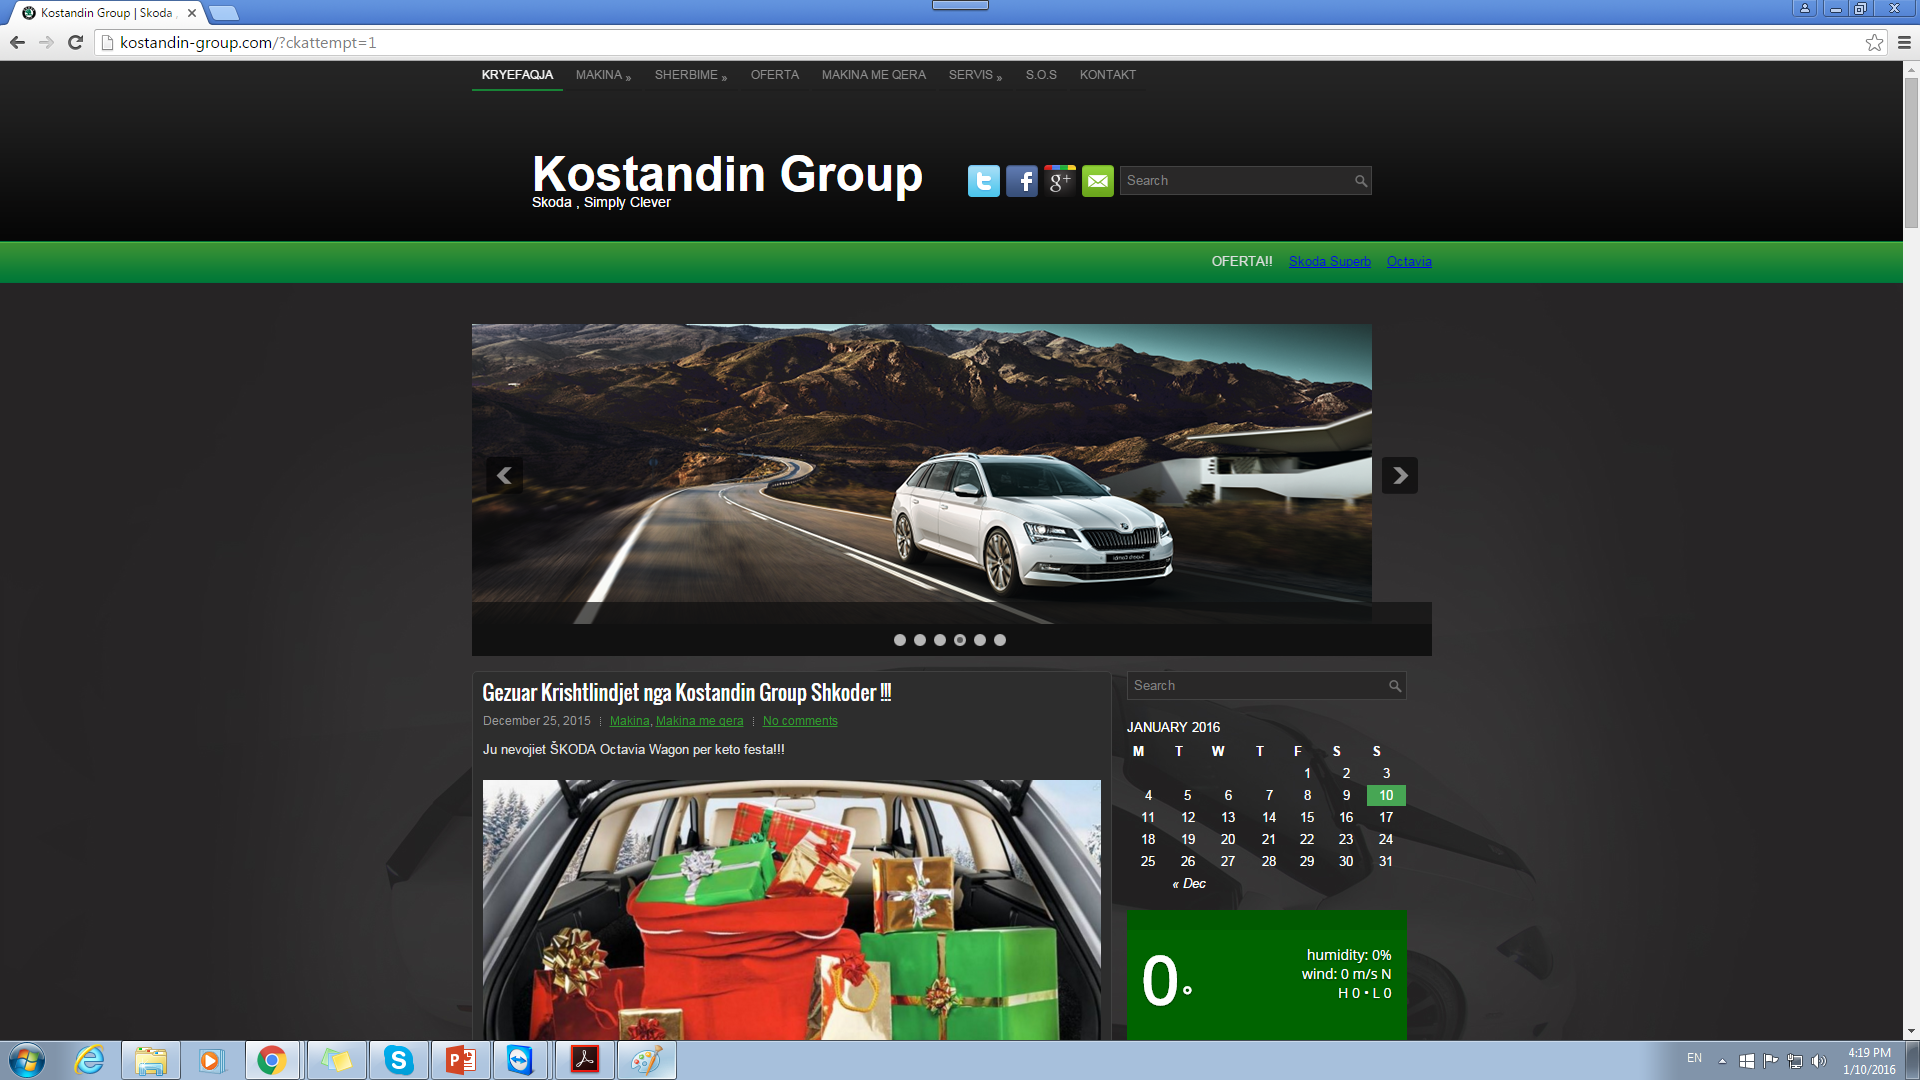
\includegraphics[scale=0.3]{Kryefaqja.png} \\
\\
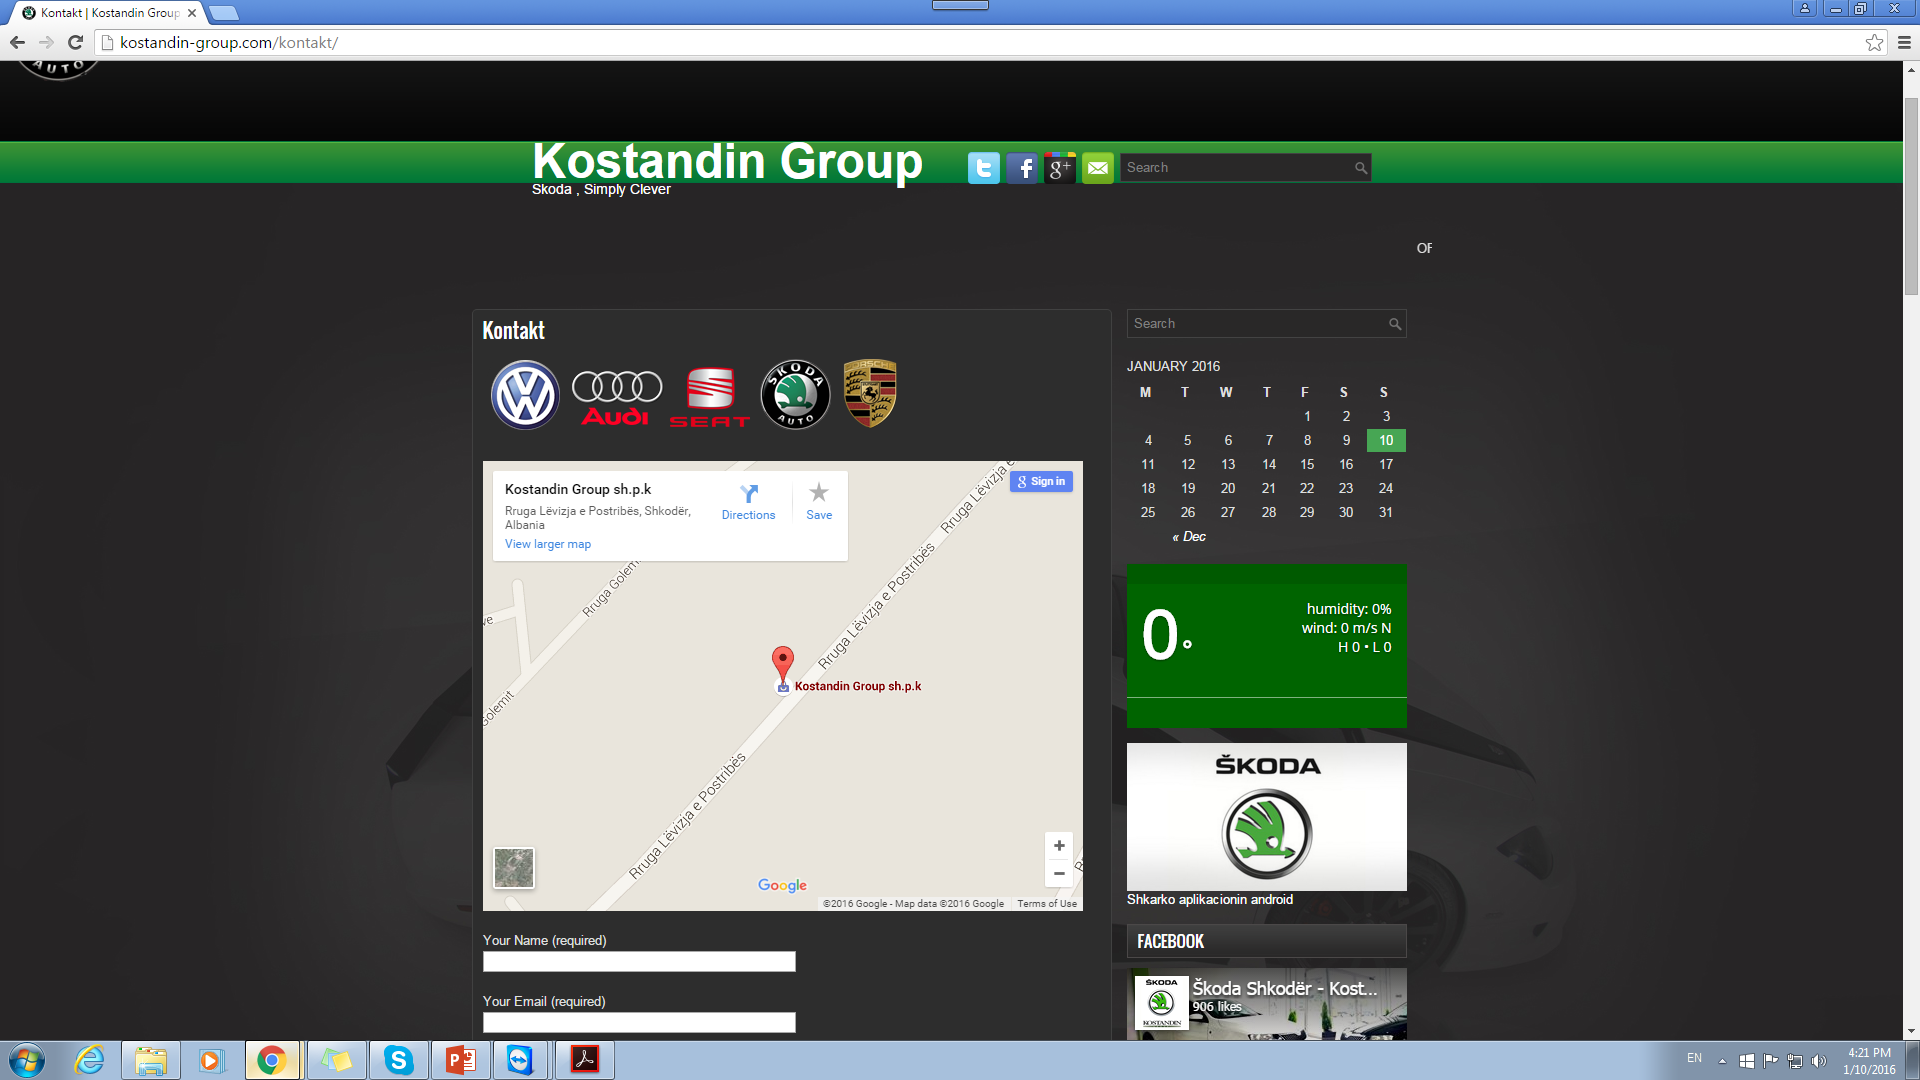
\includegraphics[scale=0.3]{Kontakt.png} \\
\\
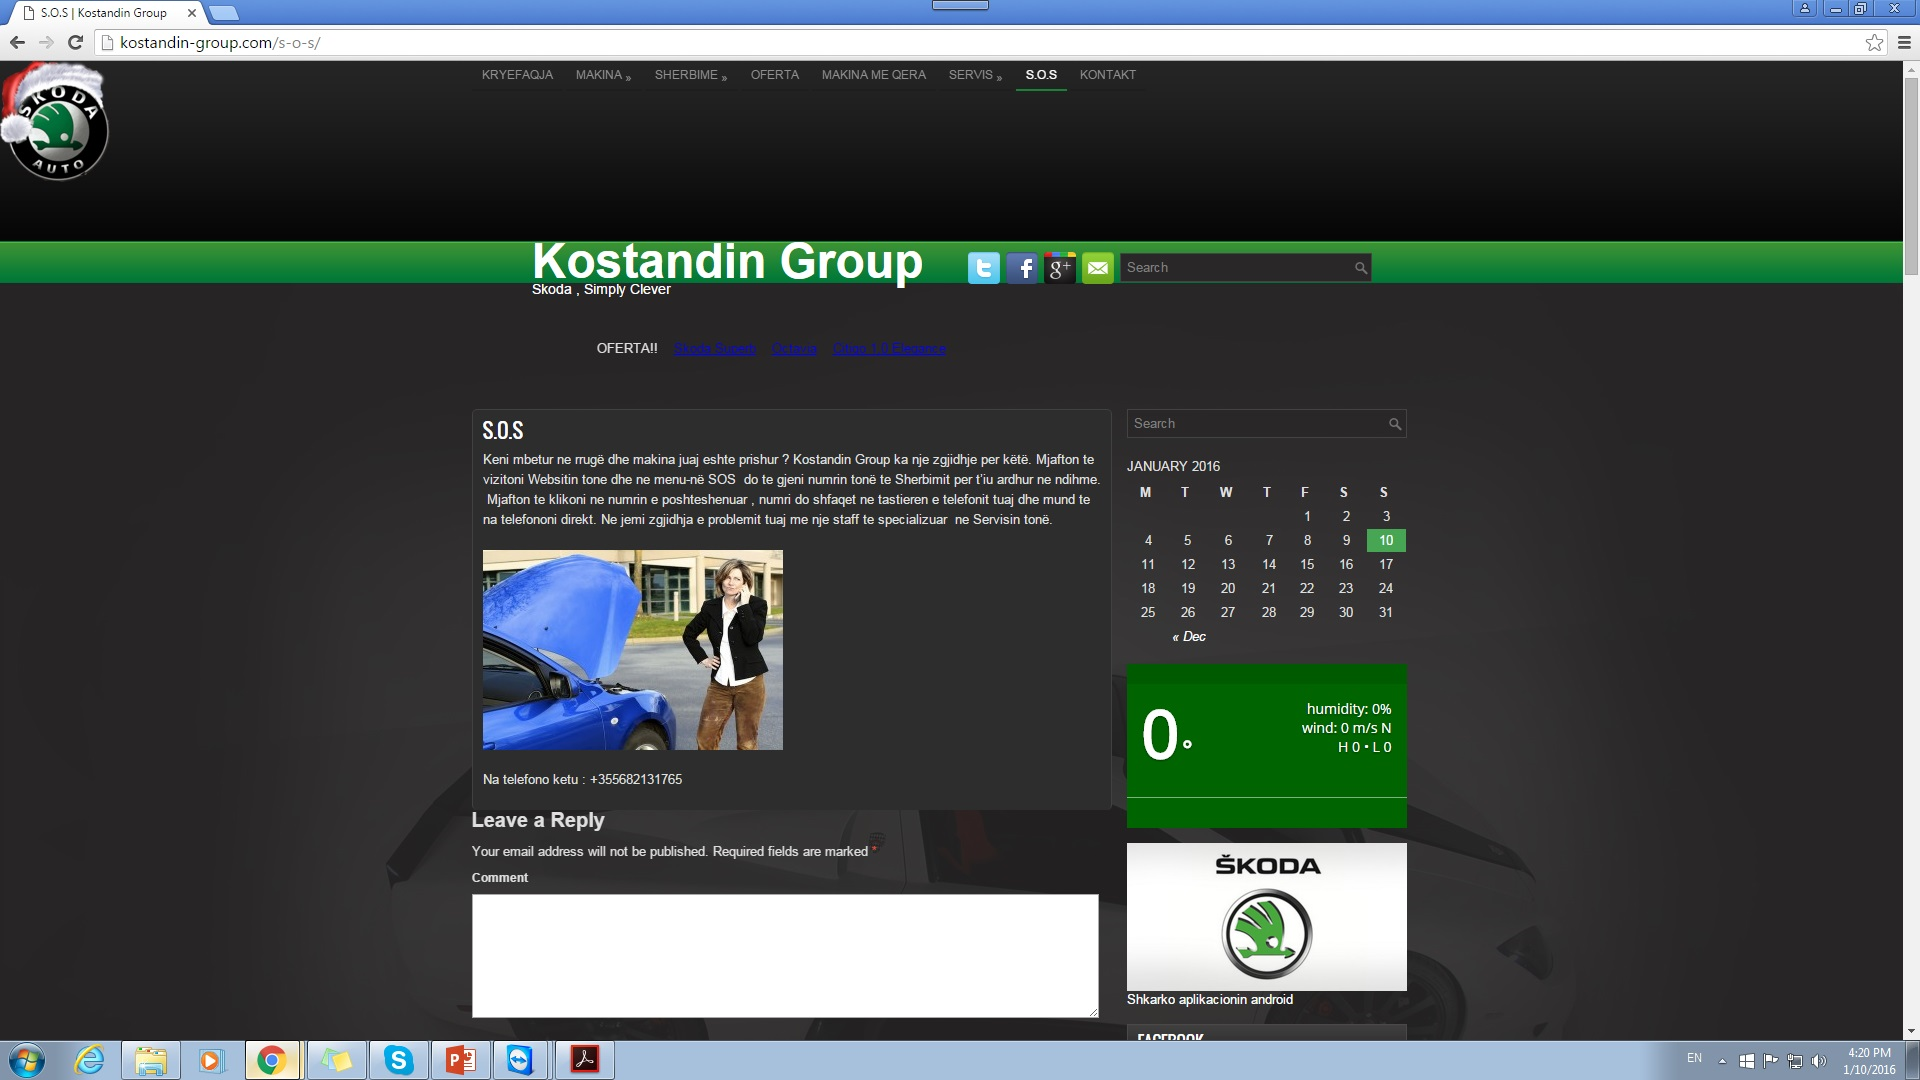
\includegraphics[scale=0.3]{SOS.png}



Die Hotspot-Zone:
Alle in Shkodra sollen wissen, wer 'Kostandin Group Skoda Shkoder' ist und was sie machen. Zu Werbezwecken wird f\"ur die Firma ein gratis Hotspot eingerichtet. Beim Verbinden mit dem Hotspot \"offnet sich als Startseite die aktuelle Firmenseite. Die Zone wo wir den Router eingesetzt haben ist in der Fussgangzone, eine Zone, die von viele Menschen jeden Tag frequentiert ist.

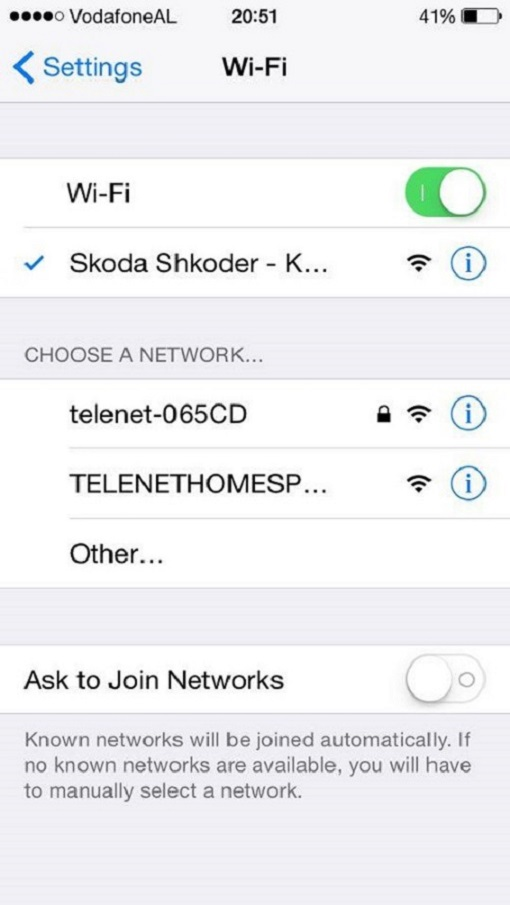
\includegraphics[scale=0.3]{HS1.jpg} 

\includegraphics[scale=0.3]{HS2.png}

\includegraphics[scale=0.3]{HS3.jpg}

Der Server:
Um die Arbeit der Mitarbeiter der Firma zu erleichtern, haben wir gedacht, ein Server aufzubauen. Die Aufgabe des Server wird die Computers miteinander zu verbinden damit die Mitarbeiter ihre Dateien zentral abspeichern und miteinander teilen. Wir sind noch nicht fertig mit dem Aufbau des Servers aber wir haben den gr\"ossten Teil der Arbeit gemacht und in manche Tagen werden wir fertig sein.

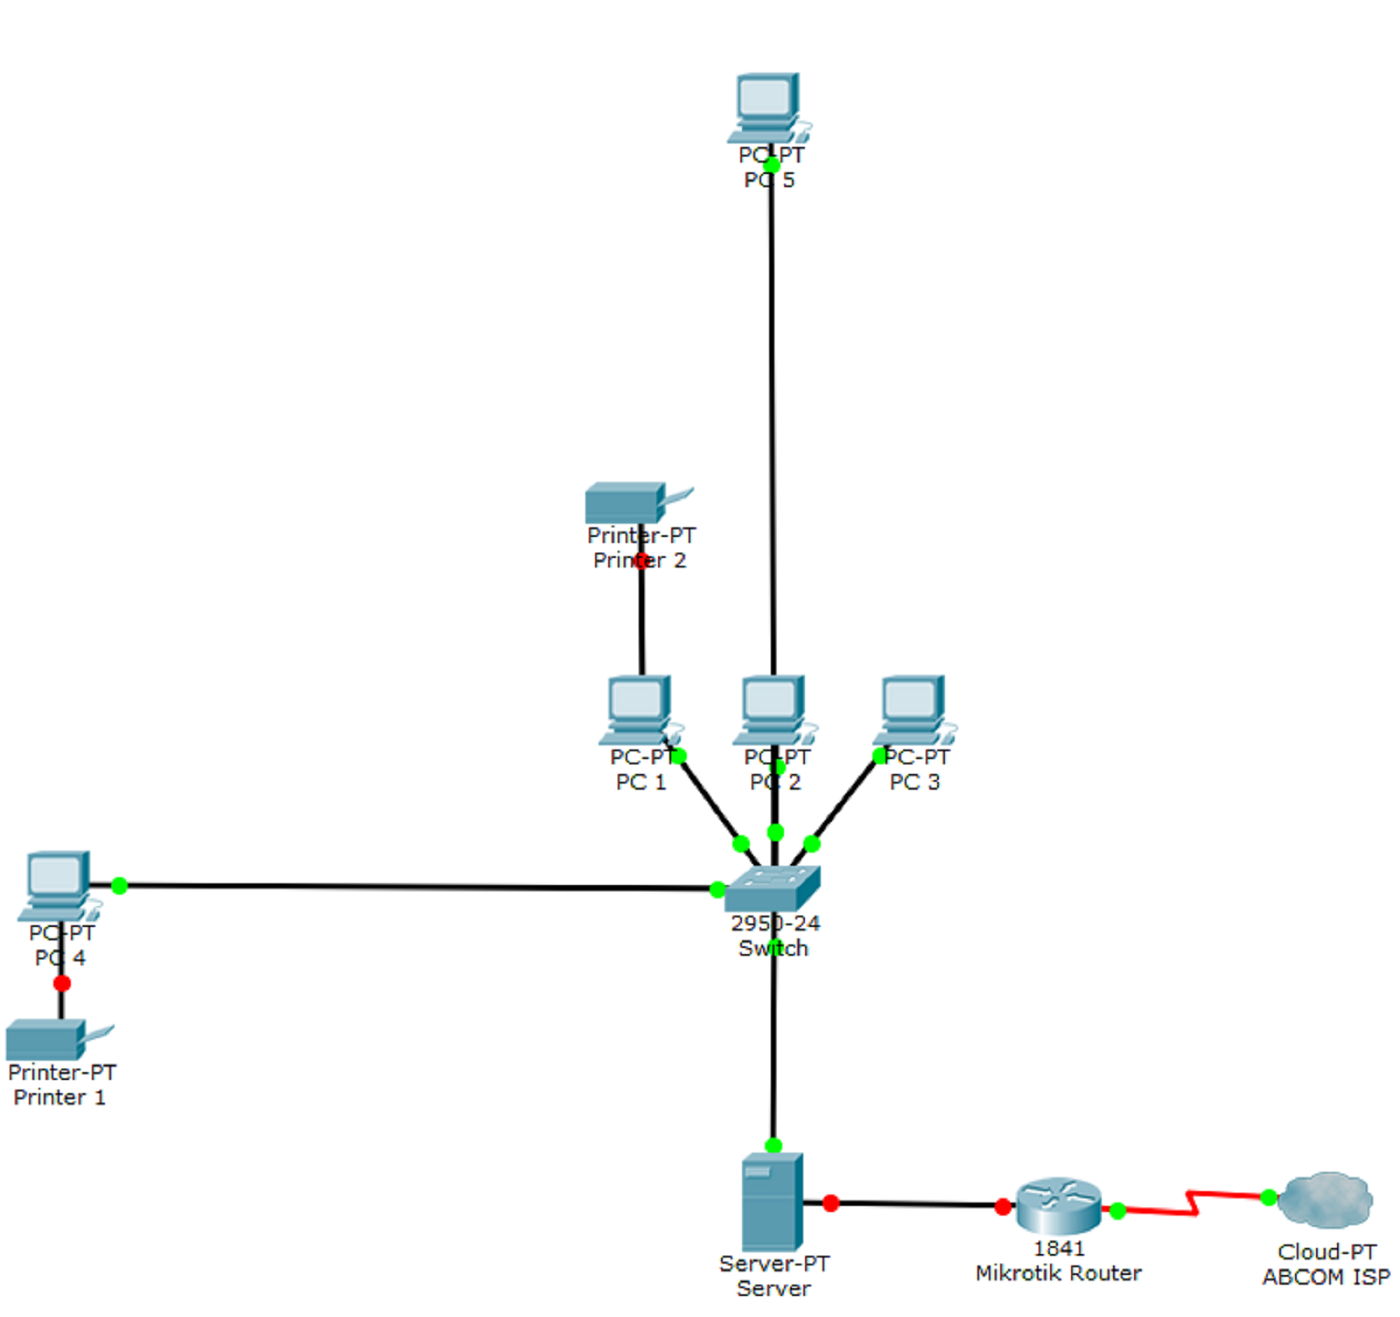
\includegraphics[scale=0.3]{server.png}

Installation und Inbetriebnahme eines Bilanzprogramms, eines Lagerprogramms und eines Rechnungsmanager:
Diese Programme werden die Arbeit der Mitarbeiter viel erleichtern, digitalisieren und schneller Machen. Dort wurden die Kunden gespeichert, die Rechnungen gemacht, alle Teilen gespeicher, der Bilanz jedes Monat gemacht usw. F\"ur die Programme haben wir zwei M\"oglichkeiten: Entweder w\"ahlen wir Open-Sources oder den Programm die von uns erstellt wird. Wir haben unser Programm noch nicht fertig gemacht und nach dem wir es fertig Machen, entscheiden wir, ob wir die Open Sources oder unser Programm verwenden werden

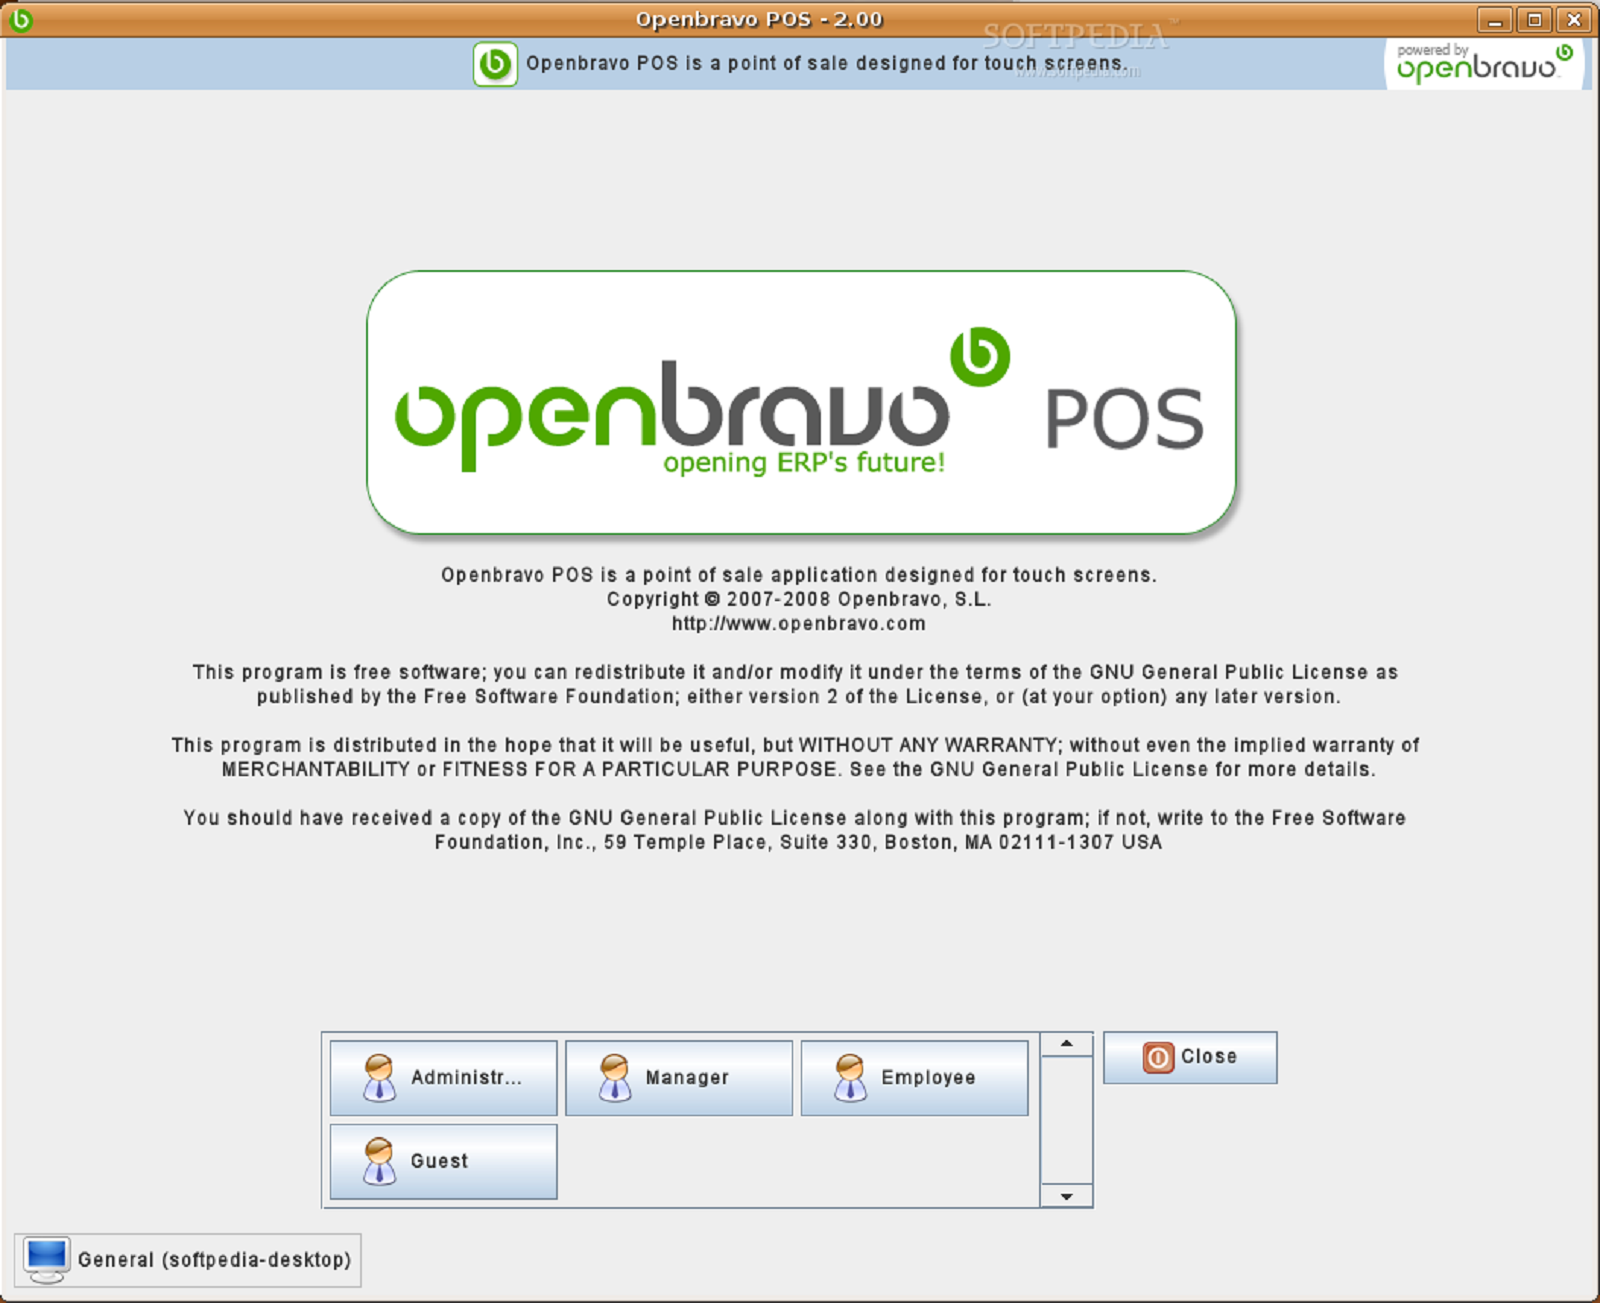
\includegraphics[scale=0.3]{prog1.png} \\
\\
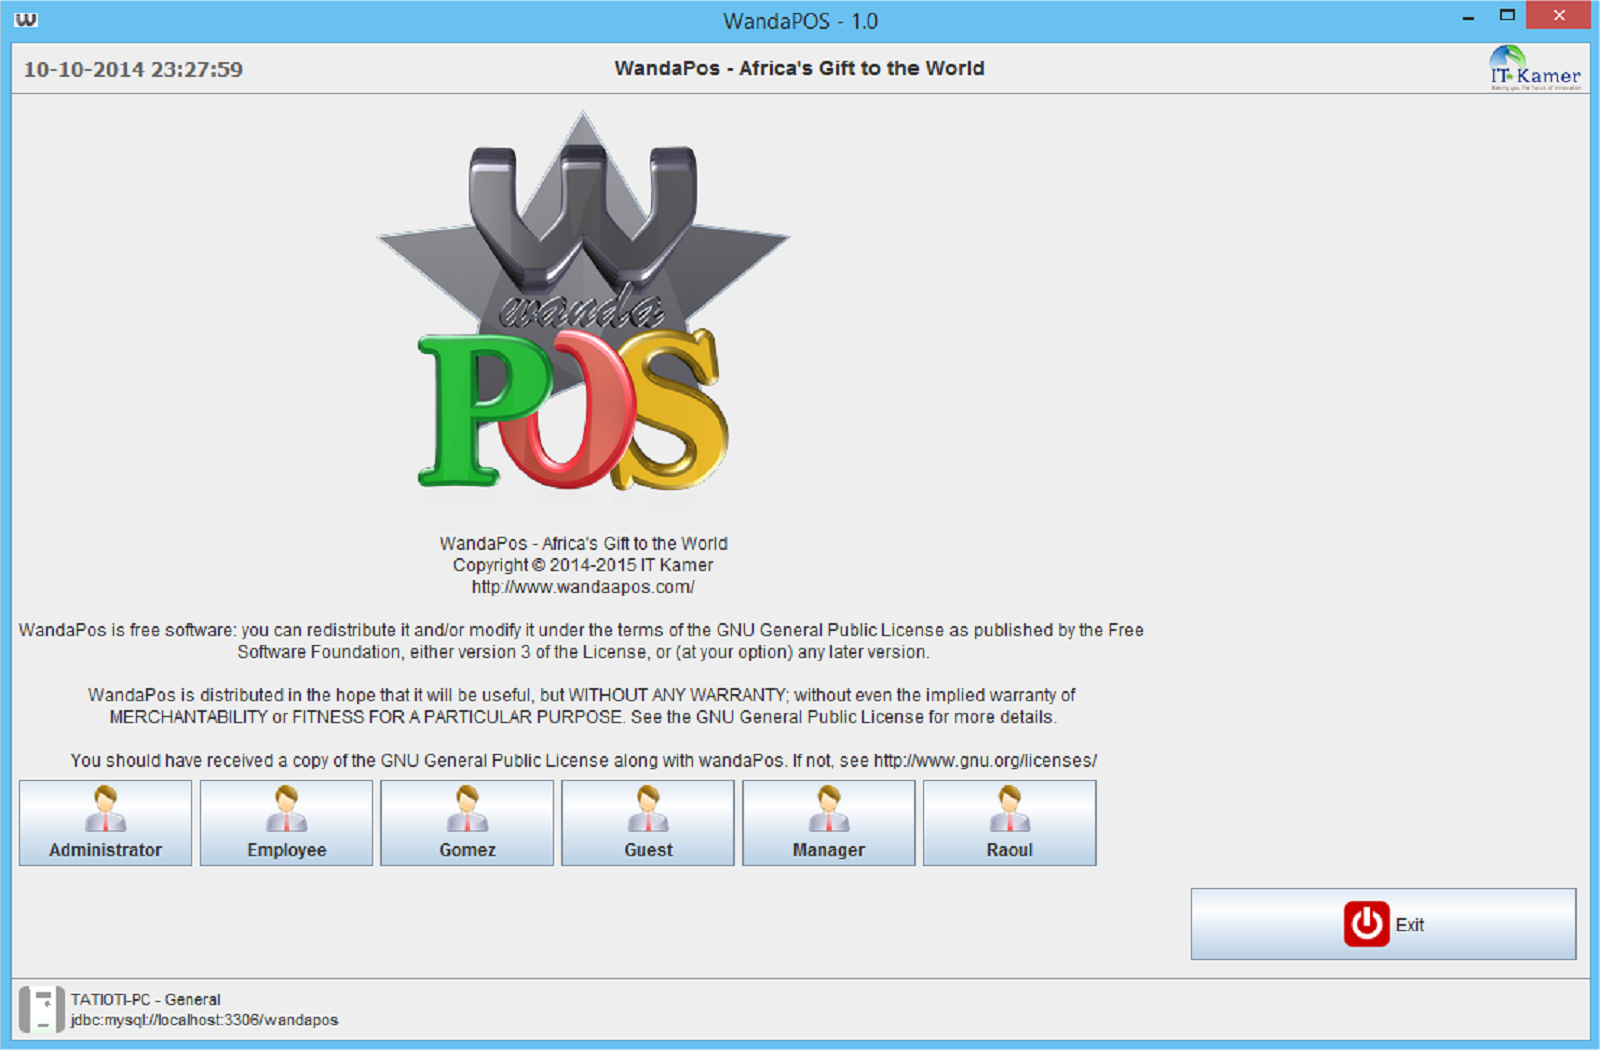
\includegraphics[scale=0.3]{prog2.png} \\
\\
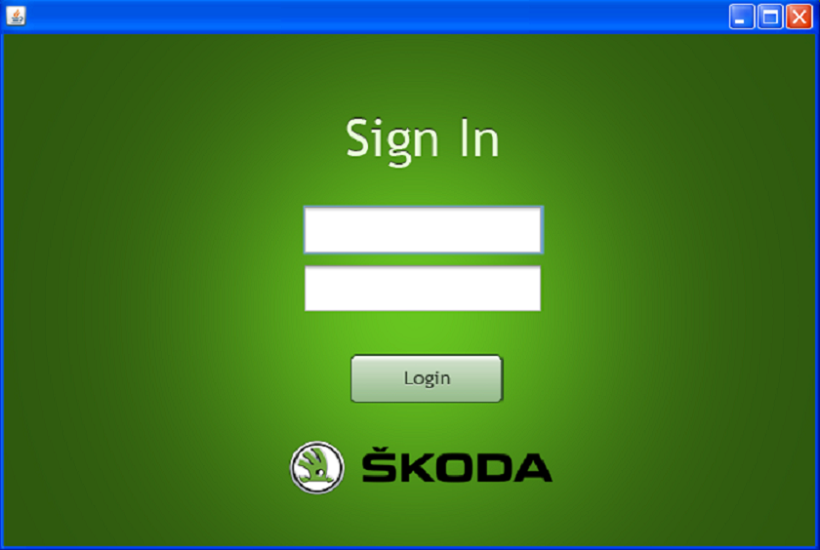
\includegraphics[scale=0.3]{prog5.png}
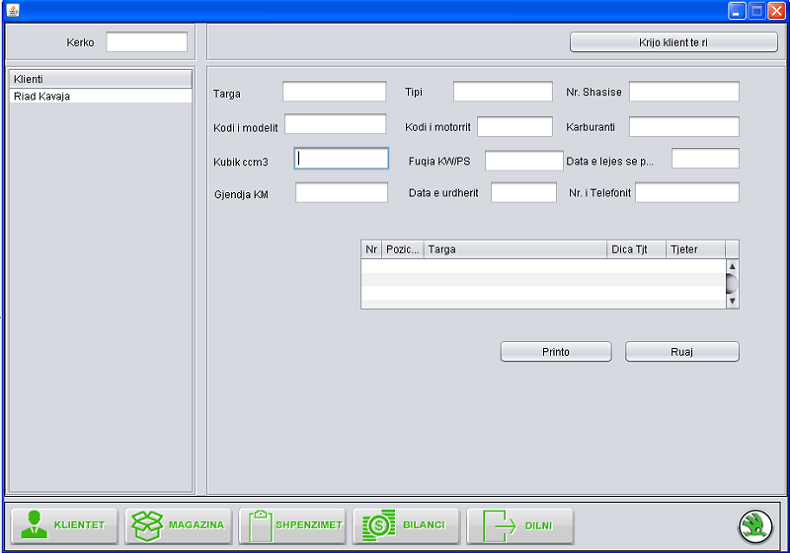
\includegraphics[scale=0.3]{prog6.png} \\
\\
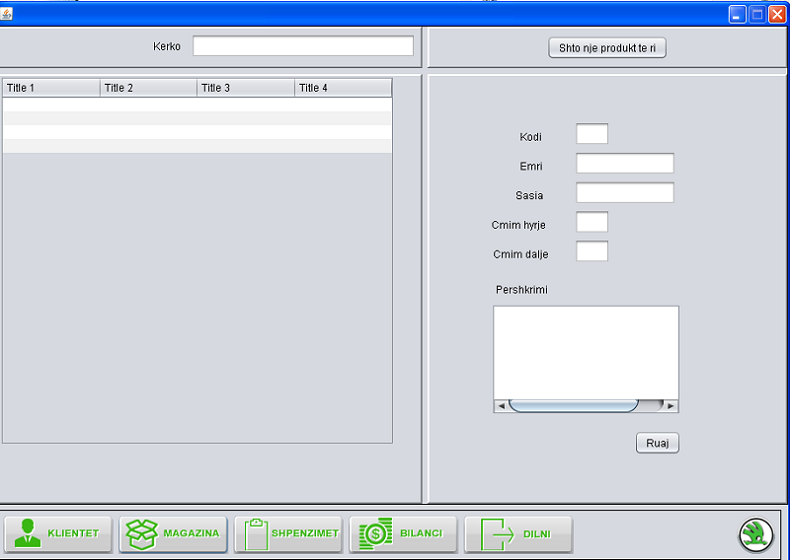
\includegraphics[scale=0.3]{prog7.png} 

Soziale Medien:
Zu Werbezwecken haben wir auch die Soziale Medien gepflegt und verbessert. Wir haben die Facebook-Fanpage verbessert, und Konten in Instagram und Google+ erstellt.

\section{Technische L\"osungen}
\subsection{Webseite}
Um die Website zu erstellen brauchten wir:
\begin{table}[ht]
\caption{Website}
\hspace*{-2cm}
\begin{tabular}{l l}
\hline\hline
Dienste & Preise \\ [0.5ex]
\hline
Domain Namecheap & 10.87 \$ \\
\hline
Host Hostgator & 8.9 \$ pro Monat \\
\hline
Wordpress & Frei \\
\hline
FileZilla & Frei \\
\hline
Themen & Frei \\
\hline
Plugins & Frei \\
\hline
\end{tabular}
\label{table:website} 
\end{table}
\\
Die Webseite haben wir durch diesen Schritte erstellt: \\
Domain wurde von Namecheap gekauft   \\
Host wurde von Hostgator gekauft \\
Wordpress heruntergeladet \\
Mit FTP Verbindung durch Filezilla sind  in Host \\
Database erstellt \\
Wordpress konfiguriert \\
Themes und Plugins installiert \\
CSS verwendet \\
Seite ver\"ofentlicht und Posts hinzugef\"ugt \\

\subsection{Die Hotspot-Zone}
Um die die Hotspot-Zone zu erstellen brauchten wir:

\begin{table}[ht]
\caption{Die Hotspot-Zone}
\hspace*{-2cm}
\begin{tabular}{l l}
\hline\hline
Dienste & Preise \\ [0.5ex]
\hline
Router & 58 euro \\
\hline
USB & 7 euro \\
\hline
DD-WRT & Frei \\
\hline
Notpad++ & Frei \\
\hline
\end{tabular}
\label{table:hotspot} 
\end{table}
Die Hotspot-Zone haben wir durch diesen Schritte erstellt: \\
Den Router gekauft \\
Den geeignetes Version von DDWRT gefunden, heruntergeladen, installiert und konfiguriert. \\
Hotspot erstellt und die Name ge\"andert \\
Die Sicherheits Kode weggenommen. \\
Es wurde so konfiguriert, dass wenn man mit Wireless sich verbindet, wird eine statische Seite ge\"offnet, den wir selbst programmiert haben, und danach automatisch zur Webseite kostandin-group.com springen. \\

\subsection{Netzwerk}
Um die die Netzwerk zu erstellen brauchten wir:

\begin{table}[ht]
\caption{Netzwerk}
\hspace*{-2cm}
\begin{tabular}{l l}
\hline\hline
Dienste & Preise \\ [0.5ex]
\hline
Visio & Frei  \\
\hline
Cisco Packet Tracer & Frei \\
\hline
Visioner 3D & Frei \\
\hline
Server & 100 euro \\
\hline
Windows Server 2008 R2 & Frei \\
\hline
\end{tabular}
\label{table:hotspot} 
\end{table}


\section{Beschreibungen des Arbeitsverlaufs}

Wir haben unser Arbeit gut organisiert, gleich geteilt, und wir haben r\"agelm\"assig gearbeitet, damit wir nicht sp\"at mit die Termine sind. Wir haben jede Mitwoch und Freitag 3 Stunden und nach dem Unterricht manchmal wenn wir etwas schnell machen mochten. Am Wochenenden haben wir auch oft gearbeitet. 
Wir haben Termine mit unserem Projektleiter, Herrn Michel gemacht. Wir haben ihm unseren Arbeit jede Woche pr\"asentiert und er hat uns es zu korrigieren geholfen und neue Ideen und Vorschl\"age gegeben.
Wir haben auch unser Projektauftraggeber getroffen und haben ihm was wir vis jetzt gemacht haben pr\"asentiert, wir haben ihm gefragt ob ihm es gef\"allt und ob er Vorschl\"age hat.
  
\section{Probleme, Herausforderungen und deren L\"osung}

Der Projektauftraggeber hat unsere Plannung ge\"andert, deshalb war es f\"ur uns nicht leicht, den Arbeit noch ein mal zu planen. Der in den ersten Plannung war das Netzwerk, die Programme und dann die Webseite und Pflegen der Sozialen Medien zu absolvieren und die Hotspot- Zone. Danach hat er gesagt dass am Beginn braucht er die Webseite, die Hotspot- Zone und die soziale Medien und danach das Netzwerk und die Programme. Um die Arbeit in der Termin fertig zu machen, haben wir die Arbeit noch einmal geteilt und mehr am begin gearbeitet, damit wir keine Problem mit die Termine am Ende zu haben. 

\chapter{Viertes Kapitel}
\section{Listen und Aufz\"ahlungen}

Hier mal eine Auflistung von Elementen
\begin{itemize}
 \item erstes Element
 \item zweites Element
 \item noch ein Element
\end{itemize}

Hier mal eine Aufz\"ahlung
\begin{enumerate}
 \item erster Punkt
 \item noch ein Punkt
 \item letzter Punkt
\end{enumerate}

\section{Und n\"achster Abschnitt etwas l\"anger als vorher es war}
Eine neue Seite, um auchmal die Kopfzeile zu sehen, da sie auf Seiten mit Kapitelanfang nicht erscheinen. Eine Abk\"urzung ist z.B. etc.\abk{etc.}{et cetera}.

\section{Eine Tabelle}

Hier eine Tabelle:
\begin{table}[htbp]
\centering
\begin{tabular}{l|l|l|l}
SpalteA & SpalteB & SpalteC & SpalteD \\
\midrule
InhaltA1 & InhaltB1 & InhaltC1 & InhaltD1 \\
InhaltA2 & InhaltB2 & InhaltC2 & InhaltD2 \\
InhaltA3 & InhaltB3 & InhaltC3 & InhaltD3
\end{tabular}
\caption{Beispiel einer Tabelle}
\label{tab:tabelle1}
\end{table}

Wie man in der Tabelle~\ref{tab:tabelle1} sehen kann ...

% Neue Seite
\section{Zitieren und Literaturverzeichnis erzeugen}
Zitierregeln sind der Word-Version der Diplomarbeitsvorlage zu entnehmen! \\
In der Datei \textit{bib.bib} im Verzeichnis \textit{Literatur} sind neue Eintr\"age von Literatur hinzuzuf\"ugen. Das Format kann in der \LaTeX{} Dokumentation nachgesehen werden. \\
N\"utzliche Links zum automatischen Erstellen von BibTeX Eintr\"agen:
\begin{itemize}
	\item \url{http://truben.no/latex/bibtex/}
	\item \url{http://www.ottobib.com}
	\item \url{http://www.literatur-generator.de}
	\item \url{https://scholar.google.de}
\end{itemize}

\begin{center}
\Large{!!! \\Damit das Literaturverzeichnis erstellt wird, muss auch mit dem \textbf{Befehl BibTeX} kompiliert werden.\\ !!!}
\end{center}


\subsection{Beispiele}
Die exakte Herleitung kann in \cite{Prager1961} nachgelesen werden. \\
Hier ein Zitat etwas einger\"uckt:
\begin{quote}
Das Programm TeX wurde von Donald E. Knuth, Professor an der Stanford University, entwickelt. Leslie Lamport entwickelte Anfang der 1980er Jahre darauf aufbauend LaTeX, eine Sammlung von TeX-Makros. Der Name ist eine Abk\"urzung f\"ur Lamport TeX \cite{latextug}.
\end{quote}

\section{Bilder und Referenzen}
\begin{figure}[htbp]
\centering

\includegraphics[width=0.7\textwidth]{abbildungsdatei} % Datei in "bilder/" bei LaTeX: eps, bei PDFLaTeX: jpg (o.�.) 
\caption{Titel der Abbildung} 
\label{fig:bild1}
\end{figure}

In der Abbildung~\ref{fig:bild1}\footnote{vgl. Zitat A\cite{referenzA}} % referenzA muss im Verzeichnis literatur in der Datei bib.bib enthalten sein
ist zu sehen, dass ...

\section{Formeln}
\label{sec:formeln}

\subsection{Albert Einstein}
Keine Formel der modernen Physik ist in der allgemeinen \"Offentlichkeit wohl so bekannt wie die Einsteinsche Formel:
\begin{equation*}
  E = mc^2
\end{equation*}.

\subsection{Allgemeine quadratische Gleichung}
\begin{equation*}
  ax^2 + bx + c = 0
\end{equation*}

\begin{equation*}
  x_{1/2} = \frac{-b \pm \sqrt{b^2-4ac}}{2a}
\end{equation*}

\subsection{Intergral}
\begin{equation}
  \label{eq:1}
  \int\limits_{a}^{b} x^{2} \, dx = \frac{ b^{3} - a^{3} }{3}
\end{equation}
Siehe Beispiel \eqref{eq:1} \\
Siehe Abschnitt \ref{sec:formeln}

\section{Source Code einbinden}
\subsection{Datei}
Hier eine Einbindung von Source Code in Form einer Datei (funktioniert mit allen g\"angigen Programmiersprachen):
\lstinputlisting[label=lst:helloworldjava,caption=Hello World in Java]{./src/HelloWorld.java}
Die Ausgabe am Bildschirm von Hello World in Java ist in \ref{lst:helloworldjava} zu sehen.
\subsection{Inline}
Dieser Source Code ist direkt in \LaTeX{} eingegeben:
\begin{lstlisting}[caption=Hello World in C, label=lst:helloworldc]
#include <stdio.h>

/* Block
 * comment */
 
int main()
{
    // Line comment.
    printf("Hello World\n");
 
    return 0;
}
\end{lstlisting}
Die Ausgabe am Bildschirm von Hello World in Java ist in \ref{lst:helloworldc} zu sehen.

% Setze Numerierung wieder auf roemisch zuruek und setzte von oben fort
% Wert ist demnach der von 'roemisch'
\newpage
\pagenumbering{Roman}
\setcounter{page}{\value{roemisch}}

% Literaturverzeichnis
\bibliographystyle{plain}
\bibliography{literatur/bib}

% Appendix, falls vorhanden
\appendix
% Anh�nge, beliebig, kein Zwang
\chapter{Anhang Eins}

\chapter{Anhang Zwei}
% usw ...


\end{document}
